\chapter{Robot localization using light landmarks}
\label{Appendix:lightLandmarks}
\vspace{-1cm}


\fancyfoot[CE,CO]{APPENDIX A. LOCALIZATION USING LIGHT LANDMARKS}

This appendix summarizes the work undertaken towards a new system that would allow robot localization in a controlled environment, with the use of low-cost light sensor arrays on board each robot, in combination with purposely placed luminous landmarks.
The scenarios, data generation and techniques used for data processing are explained, and the resulting implementation is evaluated.


\subsection*{Landmark localization approach}

The proposed system would consist in stationary light sources whose position within the monitored area is known.
With a simple sensor array (shown in Fig. \ref{fig:lightLandmarks/LDR_sensor_array}), a robot would then be able to identify the direction and distance of each light source in order to infer its relative position in the environment.
As the utilized sensors were low-cost, the implementation of this technique required the calibration of the light sensor responses and the creation of adaptable models. For instance, the attenuation of light due to distance (Fig. \ref{fig:lightLandmarks/LDR_intensityVSdistance}) was modeled with exponential curve fitting in order to linearize the sensor responses.









\begin{figure}[h!]
\centerline{\mbox{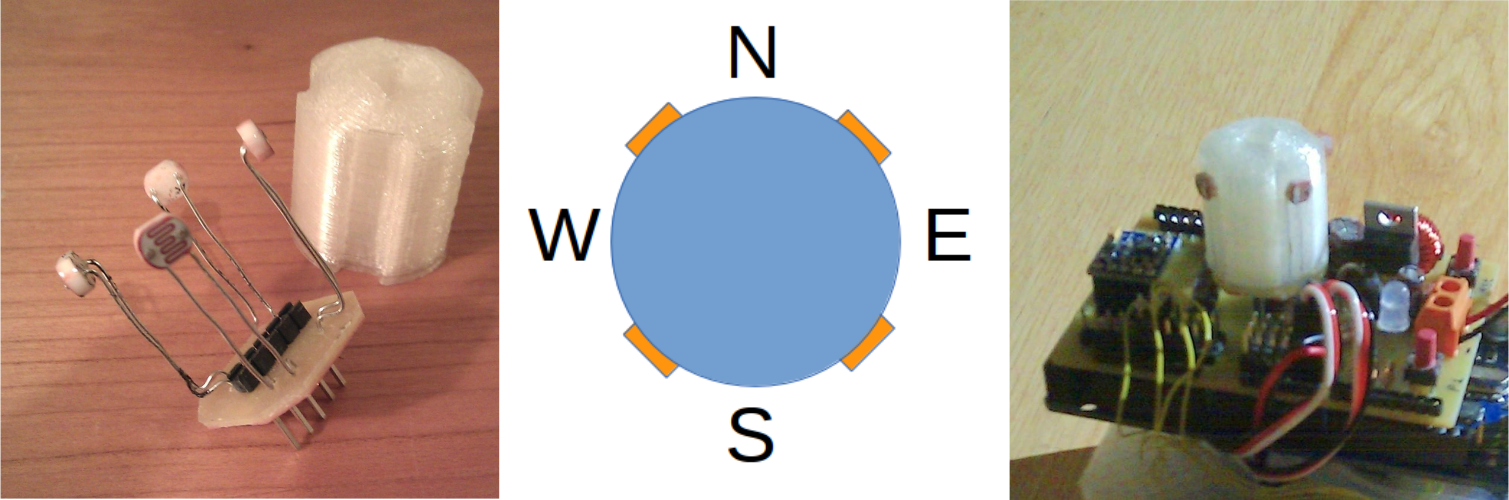
\includegraphics[width=15cm]{images/lightLandmarks/LDR_sensor_array.eps}}}
\captionFigure{Low-cost light sensor array for light-based landmark localization}
{fig:lightLandmarks/LDR_sensor_array}{
Light sensor array (left), position diagram (middle) and array mounted in a GNBot (right).
The light sensor array is made of four light-dependent resistors arranged in a ring shape. These are held in position using a 3D-printed shape designed for the purpose, and can be easily connected to the GNBoard electronics. The output is measured as a 10 bit ADC value [0-1023] that is proportional to the resistance.
}\end{figure}






\begin{figure}[h!]
\centerline{\mbox{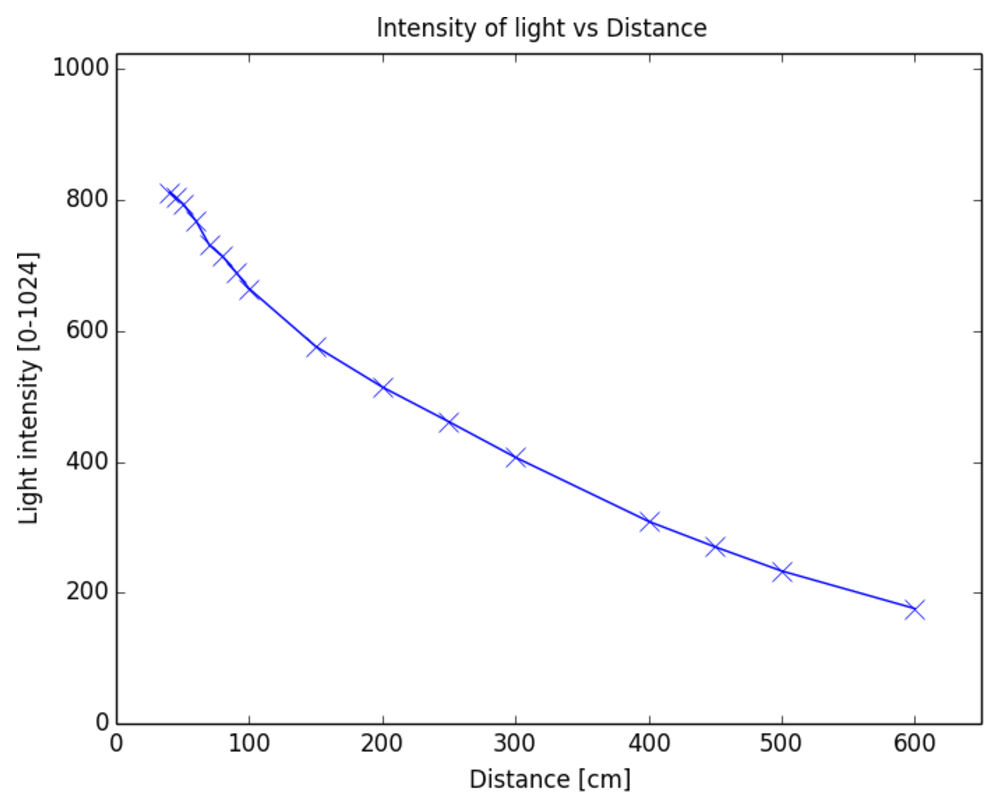
\includegraphics[width=9cm]{images/lightLandmarks/LDR_intensityVSdistance.eps}}}
\captionFigure{Response curve of the light sensors utilized}
{fig:lightLandmarks/LDR_intensityVSdistance}{
The figure shows the measured response of a light sensor at 16 different distances from a light source.
By modeling this response curve it is possible to later infer the distance of a perceived light source.
Details on the employed sensor can be found in Fig. \ref{fig:lightLandmarks/LDR_sensor_array}.
}\end{figure}







\subsubsection{Data generation for light source modeling}


The motion of the robot was restricted to be a rotation over the XY plane to simplify the initial light source modeling experiments. This decision was made since the swarm of robots would be operating in a 2-D environment. By restricting the motion to a rotation, it is possible to evaluate the light intensity measurements more easily. The experiments are described in Figure \ref{fig:lightLandmarks/GNBot_light_landmarks}.

\begin{figure}[h!]
\centerline{\mbox{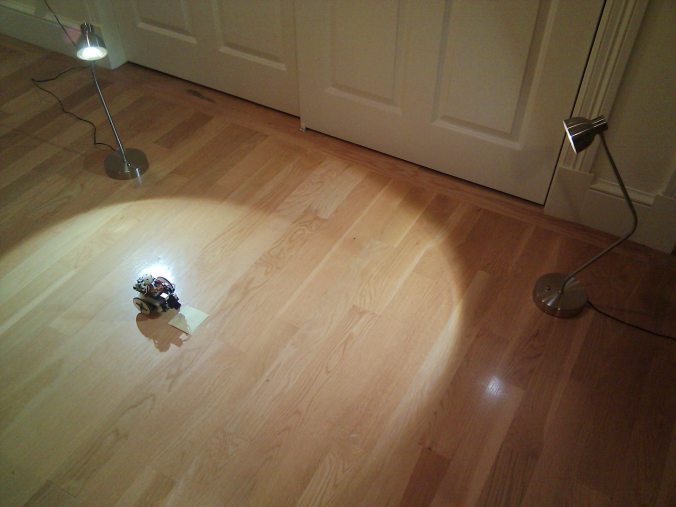
\includegraphics[width=10cm]{images/lightLandmarks/GNBot_light_landmarks.eps}}}
\captionFigure{GNBot and two light-based landmarks}
{fig:lightLandmarks/GNBot_light_landmarks}{
For the data generation, $N$ light sources were placed in the robot's operating environment. The robot was located on a known spot, where it would make M self-turns spinning at a constant speed while logging the following data:
\vspace{-0.3cm}
\begin{packed_enum}
	\item Intensity of light measured by each sensor of the array
	\item Angle of rotation of the robot measured with the electronic compass
\end{packed_enum}
\vspace{-0.3cm}
At the end, the goal was to determine the direction (angle) and distance to each of the light sources.
}\end{figure}



After some initial tests, a number of measurements were conducted. Each test was repeated both with ambient light and in the dark, with M = 3 full rotations for each experiment.
%\vspace{-0.3cm}
%\begin{packed_enum}
%	\item No light focuses
%	\item One light focus (bright) 
%	\item Two light focuses (both bright) - shown in Fig. \ref{fig:lightLandmarks/GNBot_light_landmarks}
%	\item Three light focuses (two bright, one dim)
%	\item Four light focuses (two bright, two dim)
%\end{packed_enum}
%\vspace{-0.3cm}
One light focus was added at a time, and all the parameters of the experiment (real position of each light, amount of ambient light, and all of the sensor responses) were logged in real time using a Python script.
The measurements did not have any significative noise, so no pre-filtering was required, and Matplotlib was used to represent the data (see Fig. \ref{fig:lightLandmarks/LDR_rawData_experiments}).


\begin{figure}[h!]
\centerline{\mbox{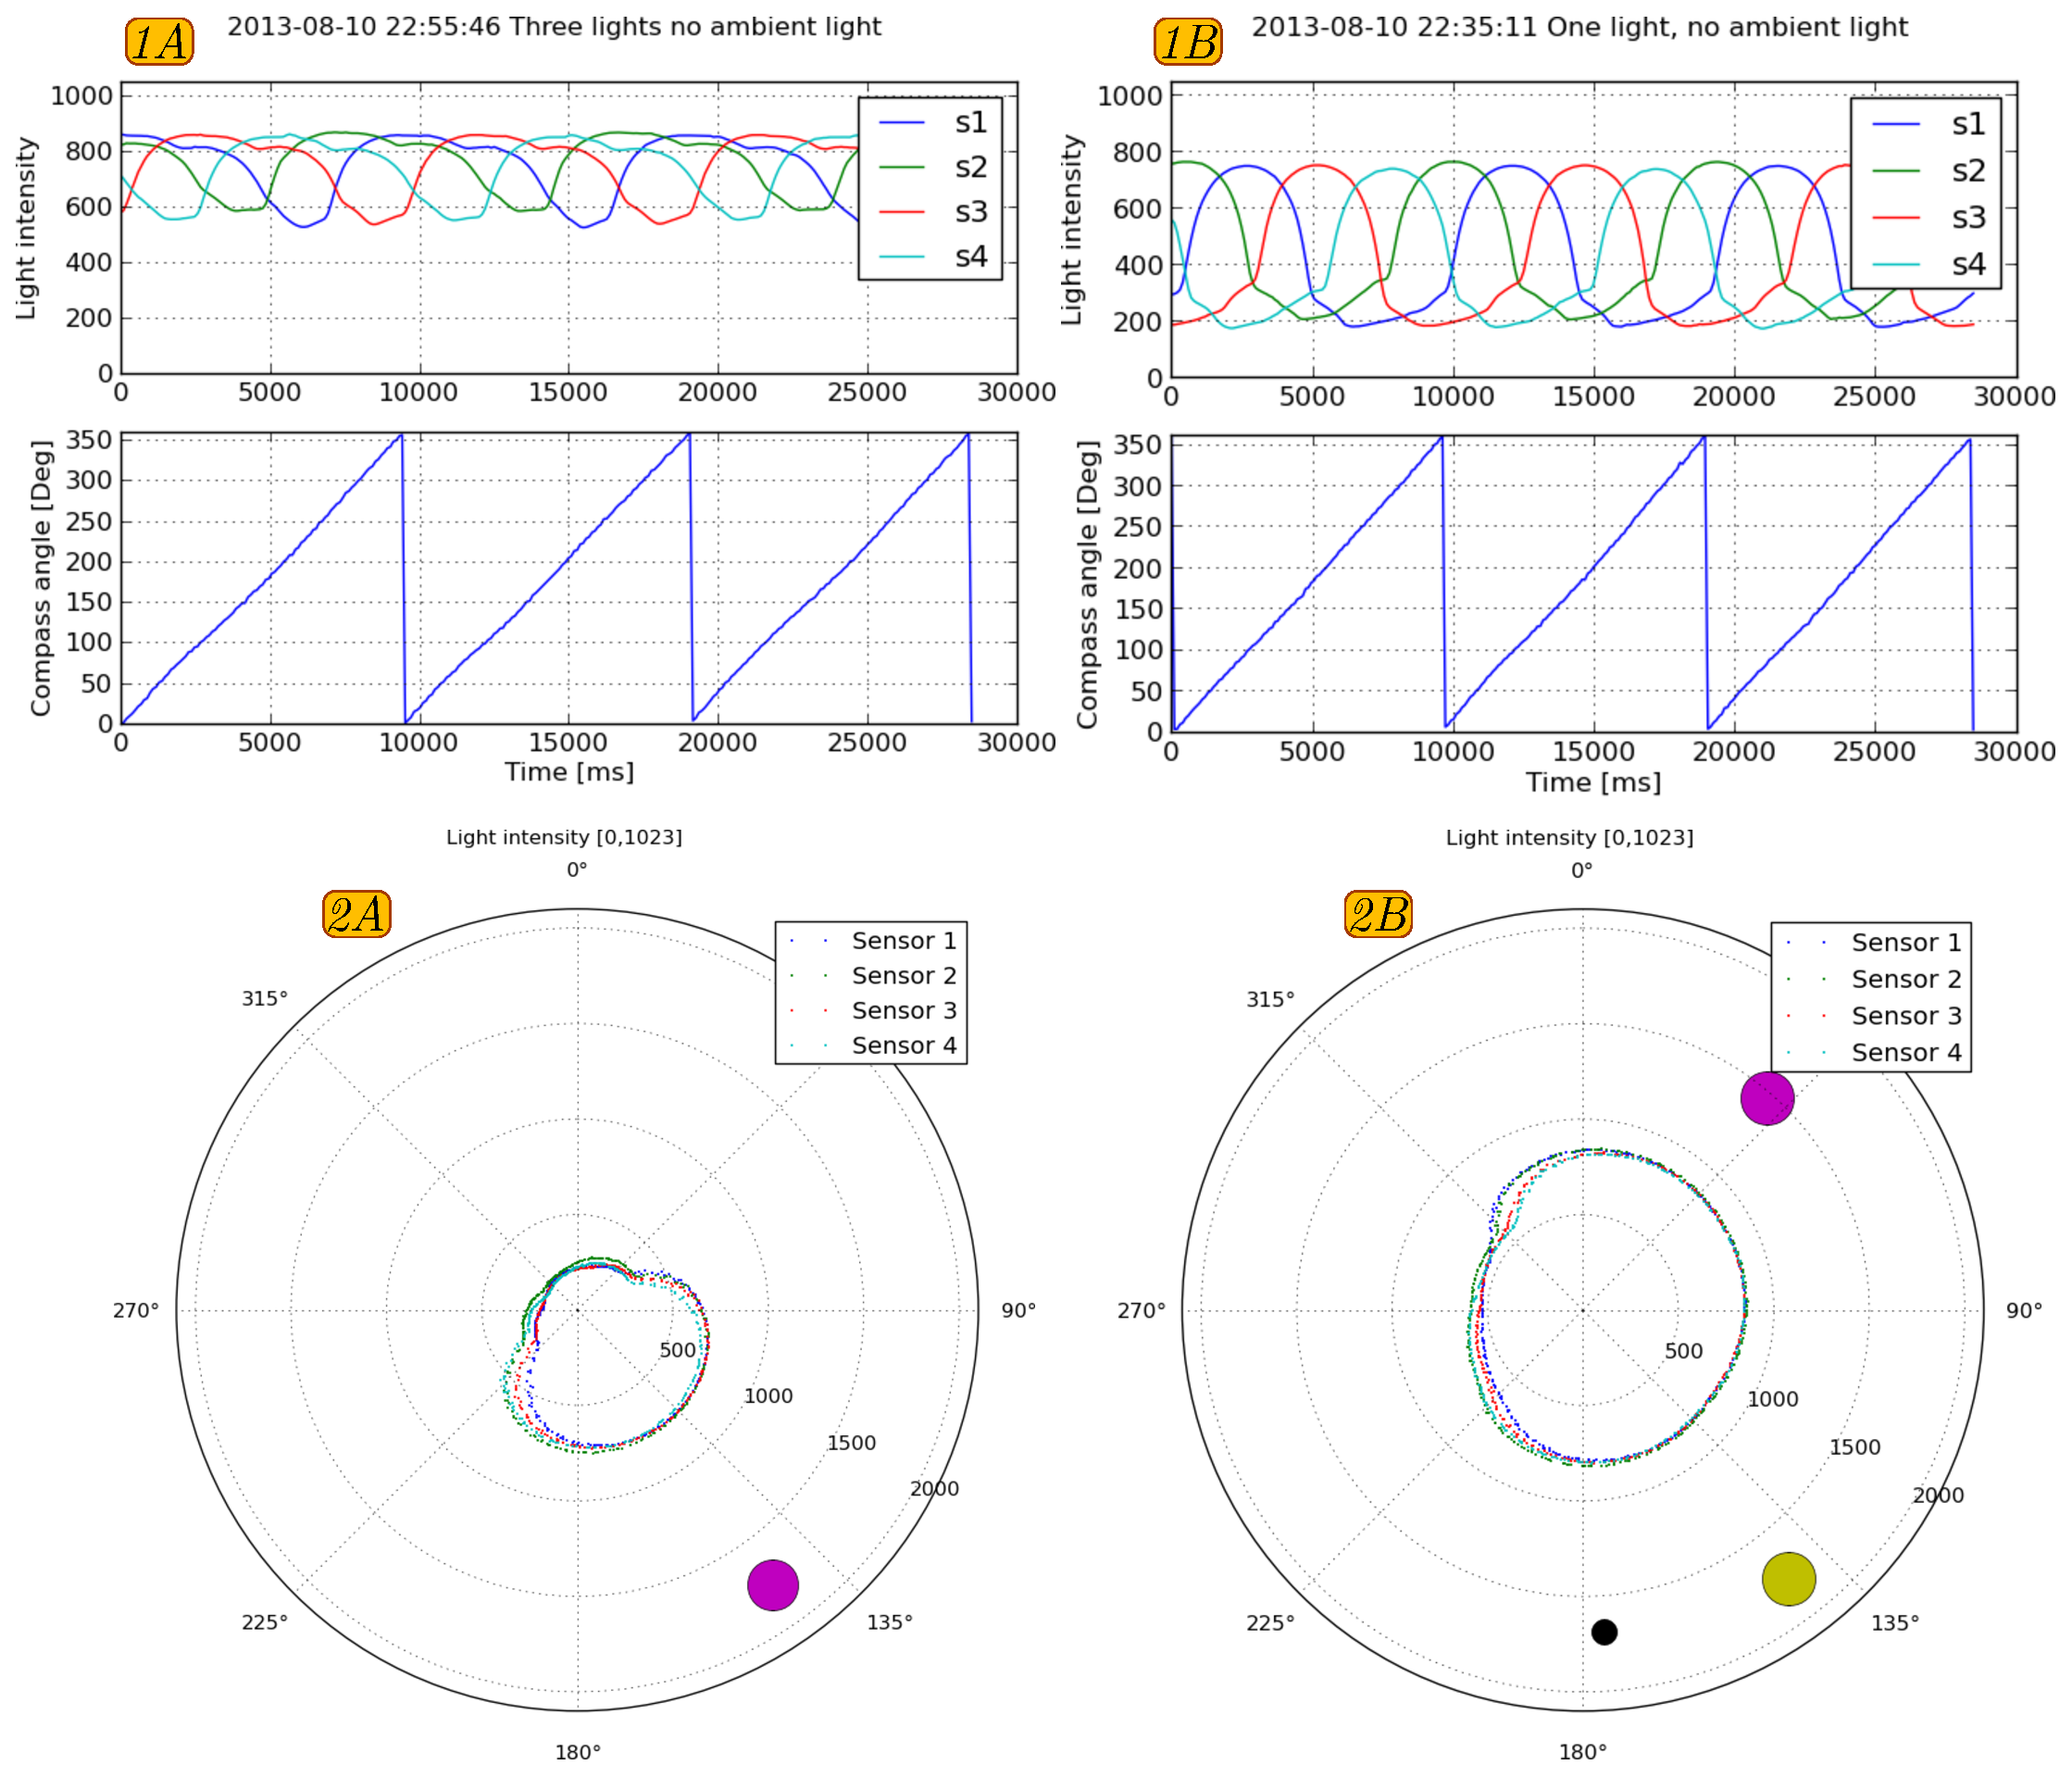
\includegraphics[width=17cm]{images/lightLandmarks/LDR_rawData_experiments.eps}}}
\captionFigure{Data from two different light landmark measurements}
{fig:lightLandmarks/LDR_rawData_experiments}{
\emph{1.A} and \emph{1.B} show the raw data from the two experiments.
\emph{2.A} and \emph{2.B} show the same data with a polar representation.
The actual position of light sources appears as colored circles.
Polar representation was preferred since the temporal dimension did not provide significative information as light sources were time invariant.
}\end{figure}




\subsubsection{Modeling the light-based landmarks}

As the intensity values are recording among an orientation measure (in degrees), the datapoints presented periodicity and thus required special polar treatment (see Fig. \ref{fig:lightLandmarks/LDR_polyfitVSfft}).




%\subsubsubsection{Polar data sampling and smoothing}


\begin{figure}[h!]
\centerline{\mbox{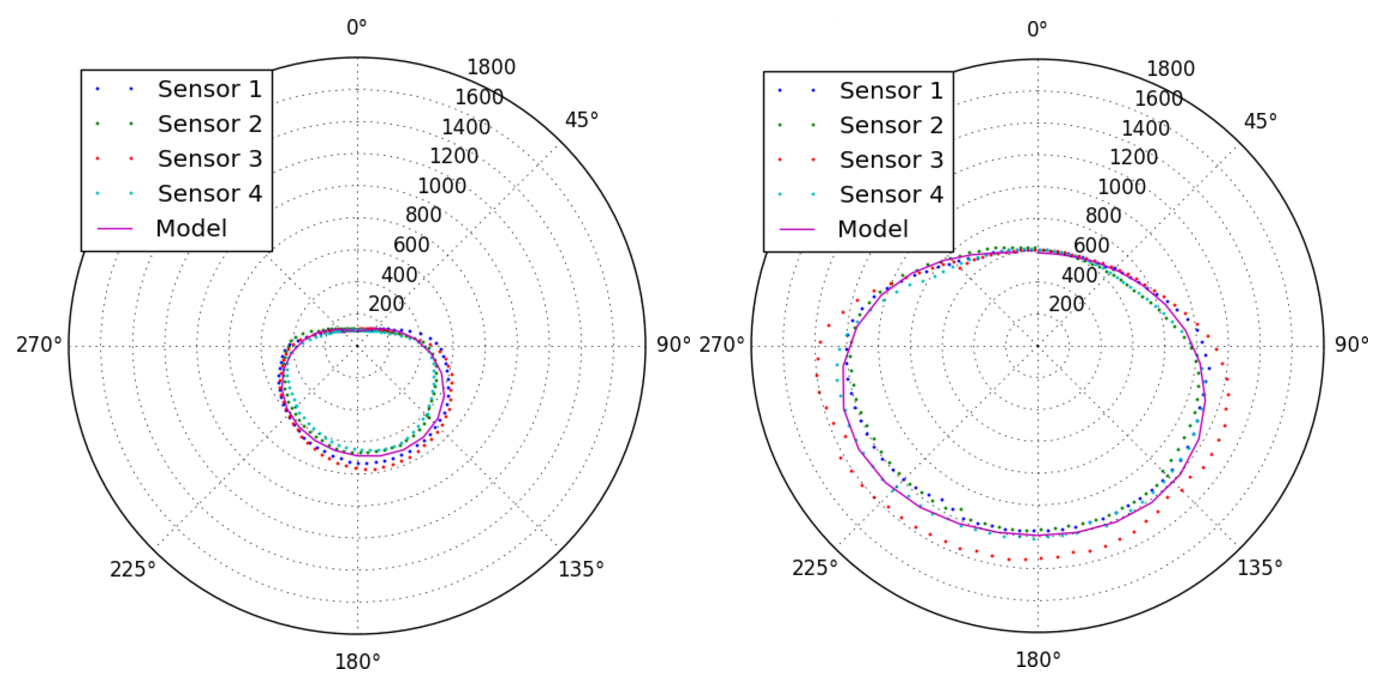
\includegraphics[width=15cm]{images/lightLandmarks/LDR_polyfitVSfft.eps}}}
\captionFigure{Smoothing the polar data using FFT low-pass filtering}
{fig:lightLandmarks/LDR_polyfitVSfft}{
The panels show the application of an FFT low-pass filter to smooth light data measurements that are polar. As a first approach, polynomial data curve fitting was used for this task, but the resulted curves presented discontinuities. The periodicity properties of FFT provided continuous results that were more adequate for the task.
}\end{figure}



%\subsubsection{Particle filtering}

%\begin{figure}[h!]
%\centerline{\mbox{\includegraphics[width=15cm]{images/placeholder.eps}}}
%\captionFigure{Diagram showing how the light-landmark localization works}
%{fig:lightLandmarks/}{
%Description
%}\end{figure}



%\subsubsection{Light landmark localization results}


After examining all the resulting data, the selected approach was to use a single light landmark (instead of multiple lights) and to incorporate measurements from both the light sensor array and the electronic compass on board the GNBot.
By measuring its global orientation and the perceived direction to the light source, the robot could then infer its relative position to the landmark (see Fig. \ref{fig:lightLandmarks/LDR_particleFilter_results}).


\begin{figure}[h!]
\centerline{\mbox{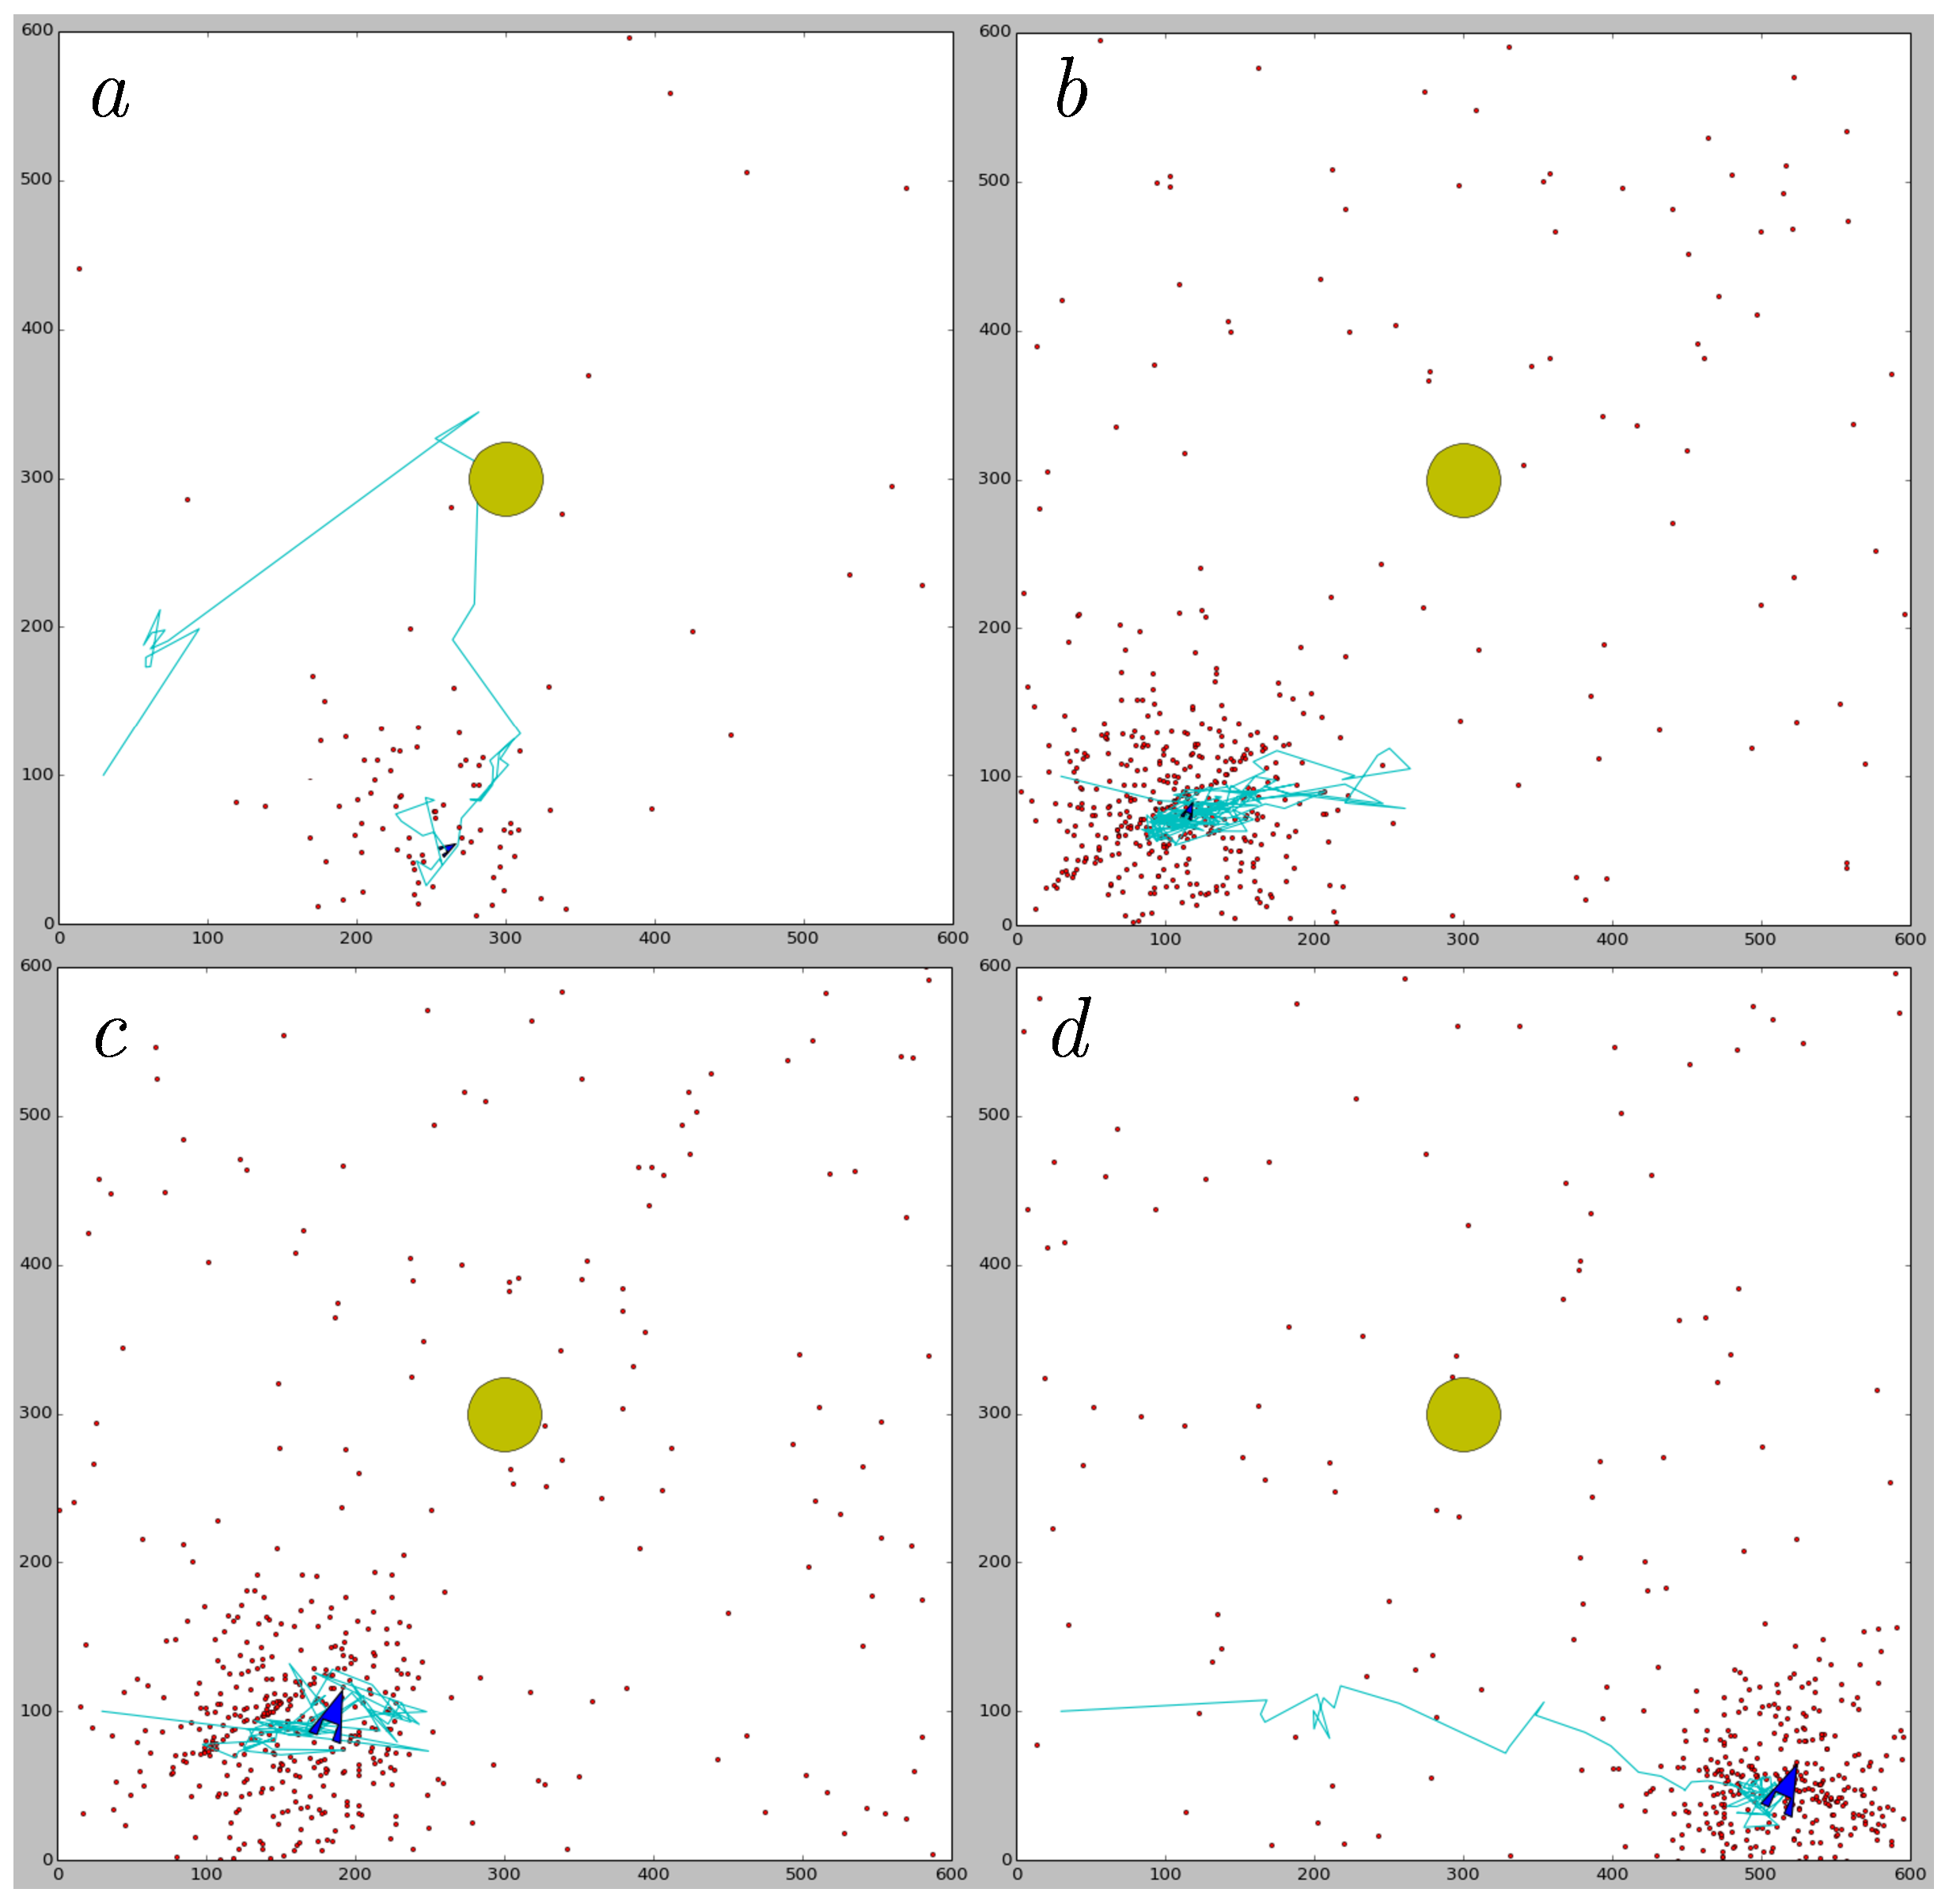
\includegraphics[width=14cm]{images/lightLandmarks/LDR_particleFilter_results.eps}}}
\captionFigure{2-D position estimation based on a light landmark}
{fig:lightLandmarks/LDR_particleFilter_results}{
The panels show data from various real robot localization experiments involving a particle filter in combination with measurements from the light sensor array and the electronic compass. Scale is in centimeters. The results have a lot of noise, because of the poor stability of the magnetic field measurement indoors.
}
\end{figure}

The implemented system performed with reasonable accuracy in simulations, but the electronic compass did not perform as expected and made the real world implementation very unreliable (specially when compared with the accuracy of the vision-based tracking system implemented in Section \ref{sect:visionBasedLocalization}).
The problem was that building floors usually have metal structures underneath, so the magnetic field is particularly distorted at low heights. Since the robots are quite low-profile, the magnetometer is then too strongly influenced by the presence of metals in the floor to allow proper robot localization.

Though, this approach for light landmark modeling and localization could be of interest for certain outdoor situations such as underwater positioning, where the light from the Sun does not create much interference.


\newpage \thispagestyle{empty} % Pagina vacia 



\fancyfoot[CE,CO]{\leftmark}

